\documentclass[titlepage]{article}
\usepackage[left=15mm,right=15mm,top=1in,bottom=1in]{geometry}
\usepackage{framed}
\usepackage{imakeidx}
\usepackage{graphicx}
\usepackage{array}
%\graphicspath{{./}}
\newcolumntype{C}[1]{>{\centering\arraybackslash} m{#1cm}}

\makeindex

\title{Autonomous Pool Playing Robot\\~\\\textbf{Proof of Concept}}
\author{
	Ernest Selman\\selmae@mcmaster.ca\\1201291\\~\\\and
	Eric Le Fort\\leforte@mcmaster.ca\\1308609\\~\\\and
	Guy Meyer\\meyerg@mcmaster.ca\\1320231\\~\\\and
	Andrew Danha\\danhaas@mcmaster.ca\\1223881\\~\\\and
	Max Moore\\moorem8@mcmaster.ca\\1320009\\~\\\and
	Derek Savery\\saverydj@mcmaster.ca\\1219142\\~\\
}
 
\begin{document}
\maketitle
\tableofcontents
~\\[15mm]
\listoftables


\vfill
\begin{table}[!htbp]
\centering
\begin{tabular}{| C{3} | C{2} | C{5} | C{2.5} |}\hline
	Date			&Revision \#	&Comments						&Authors\\\hline
	14/11/2016		&0				&- Initial document creation	&Eric Le Fort\\\hline
	~				&1				&- Software section				&Max Moore\newline Eric Le Fort\\\hline
	~				&2				&- Hardware section				&Ernest Selman\newline Guy Meyer\newline Andrew Danha\newline Derek Savery\\\hline
\end{tabular}
\caption{Revision History}
\end{table}
\newpage

%List the major technical concerns/risks you have in being able to complete your project.
%For each of those, give us reasons/analysis/portions of a design/simulations etc as to why you think you will be able to overcome those problems.

\section{Introduction}
\subsection{Purpose}
\subsubsection{Definitions}
Table \ref{tab:Definitions} lists the definitions used in this document. The definitions given below are specific to this document and may not be identical to definitions of these terms in common use. The purpose of this section is to assist the user in understanding the requirements for the system.
\begin{table}[h!]
\centering
\caption{Definitions}
\begin{tabular}{| C{6} | p{6cm} |}\hline
	\textbf{Term}	&\textbf{\centering Meaning}\\\hline
	%TODO fill in as necessary
\end{tabular}
\label{tab:Definitions}
\end{table}

\newpage
\subsubsection{Acronyms \& Abbreviations}
Table \ref{tab:Acronyms} lists the acronyms and abbreviations used in this document.
\begin{table}[h!]
\centering
\caption{Acronyms and Abbreviations}
\begin{tabular}{| p{6cm} | p{6cm} |}\hline
	\textbf{Acronym/Abbreviation}	&\textbf{Meaning}\\\hline
	%TODO fill in as necessary
\end{tabular}
\label{tab:Acronyms}
\end{table}


\section{Software Proof of Concept}
This section will outline the major technical hurdles that must be overcome in order for this project to be a success. For each case, the concern will be discussed followed by the team's plan on how to overcome that issue.

\subsection{Visual Recognition Software Usage}
For the visual recognition we need to be able to take a photo of the table, followed by having a script run that will recognize the position of balls, and finally be able to save that into a array of positions such that our decision making algorithm can operate easily and successfully. \\ \\
We felt the best way to prove that we would be able to overcome this challenge would be for us to make a matlab script that at the very least: highlighted and recorded ball positions. As we expected this proved challenging, but after some work with it we have it identifying and recording the position of lightly coloured, or well-lit balls, in the future we will have to work towards recognizing dark balls, or maybe having a better lighting situation. Having said that for now we can be confident that we can recognize stationary balls via picture. \\ \\

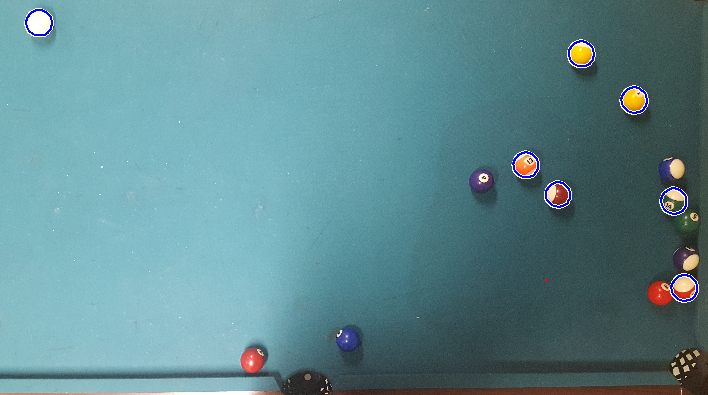
\includegraphics{gotsomeballs.PNG}
\pagebreak

Some problems that we ran into that we think we can easily solve are as follows
\begin{itemize}
\item more even lighting, so that we can better catch balls like the purple and green ball.
\item a wider angle lens, or lens attachment so that we can take photos from closer to the table.
\item some work on the algorithm so that it searches for both more relatively light and relatively dark "circles" in contrast to the background.
\item save them as a position of the table, rather than a position  in the image, this could be done with either a more cropped photo (centered relatively well on the table) or simply by having Matlab recognize the position of the table (done more easily than the recognition of the balls.) 
\end{itemize}


\subsection{Inter-Device Communication}
%TODO define facets of problem
%TODO define how we will overcome problem

\subsection{Shot Selection}
%TODO define facets of problem
%TODO define how we will overcome problem

%TODO are there more difficult sections to prove?


\section{Hardware Proof of Concept}
This section will outline the major technical hurdles that must be overcome in order for this project to be a success. For each case, the concern will be discussed followed by the team's plan on how to overcome that issue.
%TODO create subsection{CONCERN_TITLE}. For each, first outline the concern then how we plan to overcome it.
 
\section{Introduction}
\end{document}



